\documentclass[english,serif,mathserif,xcolor=pdftex,dvipsnames,table]{beamer}

\usepackage[T1]{fontenc}
\usepackage[utf8x]{inputenc}

\usetheme[informal]{s3it}
\usepackage{s3it}

\title[4. Plotting, arrays, etc.]{%
  A Short and Incomplete Introduction to Julia
}
\subtitle{\bfseries Part 4: Plotting, arrays, algebra, exceptions}
\author[R.~Murri]{%
  \textbf{Riccardo Murri} \texttt{<riccardo.murri@uzh.ch>}
  \\
  S3IT: Services and Support for Science IT,
  \\
  University of Zurich
}
\date{September 12, 2019}


\begin{document}

% title frame
\maketitle

\part{Plotting}
\begin{frame}[fragile]
  \href{http://docs.juliaplots.org/}{Plots} is the most-used plotting
  library in the Julia community.

  \+
  The most common options are summarized in
  \href{https://github.com/sswatson/cheatsheets/blob/master/plotsjl-cheatsheet.pdf}{this
    cheatsheet} by Samuel~S. Watson.

  \+ The official documentation is available at:
  \url{http://docs.juliaplots.org/latest/learning/}
\end{frame}


\begin{frame}[fragile]
  \frametitle{Preparing for plotting}

  Readying \texttt{Plots} for use is a two-step process:
  \begin{enumerate}
  \item Import the \texttt{Plots} module:
\begin{lstlisting}
~\julia~ using Plots
\end{lstlisting}
  \item Select a \href{http://docs.juliaplots.org/latest/tutorial/#plotting-backends}{visualization backend}:
    \begin{itemize}
    \item \href{http://docs.juliaplots.org/latest/examples/gr/}{GR}, a
      fast rendering backend:
\begin{lstlisting}
~\julia~ gr()  # default backend
Plots.GRBackend()
\end{lstlisting}
    \item
      \href{http://docs.juliaplots.org/latest/examples/plotlyjs/}{PlotlyJS},
      interactive visualizations (in the browser or GUI) based on
      \href{https://plot.ly/javascript/}{Plotly.js}:
\begin{lstlisting}
~\julia~ plotlyjs()  # better for notebooks
Plots.PlotlyJSBackend()
\end{lstlisting}
    \item (Other backends are available, \\ see Plots' \href{http://docs.juliaplots.org/latest/backends/}{backends} manual page.)
    \end{itemize}
  \end{enumerate}
\end{frame}


\begin{frame}[fragile]
  \frametitle{Making plots}
  The
  \href{http://docs.juliaplots.org/latest/basics/}{\texttt{plot()}}
  function is all you need to create plots:
  \begin{itemize}
  \item \alert<1>{Provide $x$-axis and $y$-axis coordinates of points;}
  \item \alert<2>{Specify how you want these drawn on the canvas.}
  \end{itemize}
\begin{semiverbatim}
\julia plot(\alt<2>{xs, ys}{\HL{xs, ys}}, \alt<1>{typ=:hline}{\HL{typ=:line}})
\end{semiverbatim}

  \+
  Note that:
  \begin{itemize}
  \item \texttt{xs} must be \emph{sorted}!
  \item \texttt{xs} and \texttt{ys} must have the same length.
  \end{itemize}
\end{frame}

\begin{frame}[fragile]
  \frametitle{Starting plots}
\begin{semiverbatim}\small
\julia xs = 0:5;
\julia ys = rand(length(xs));
\julia \HL{plot(xs, ys)}
\end{semiverbatim}
  \begin{center}
    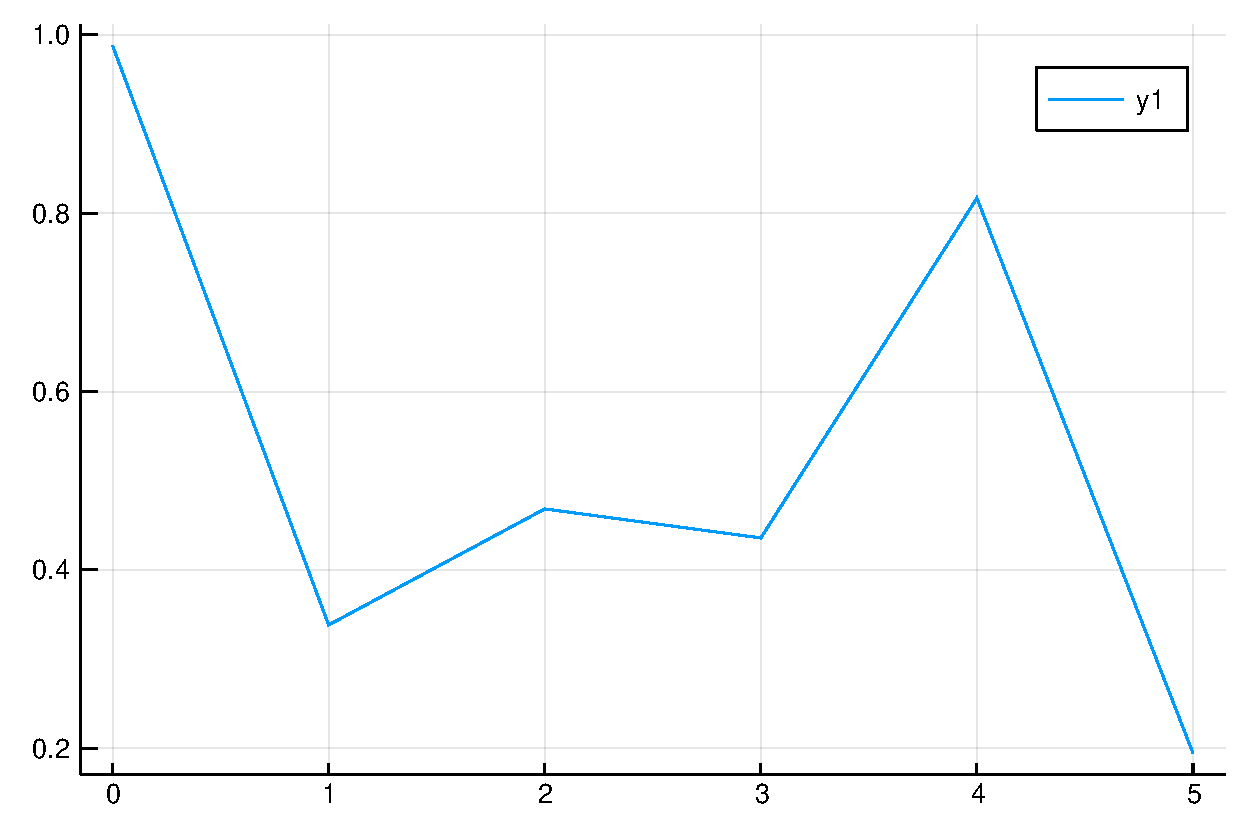
\includegraphics[height=0.66\textheight]{fig/plot1.pdf}
  \end{center}
\end{frame}


\begin{frame}[fragile]
  \frametitle{Overlaying plots, I}
\begin{semiverbatim}\small
\julia xs = 0:5;
\julia ys = rand(length(xs));
\julia plot(xs, ys)
\julia \HL{plot!(xs, ys, typ=:scatter)}
\end{semiverbatim}
  \begin{center}
    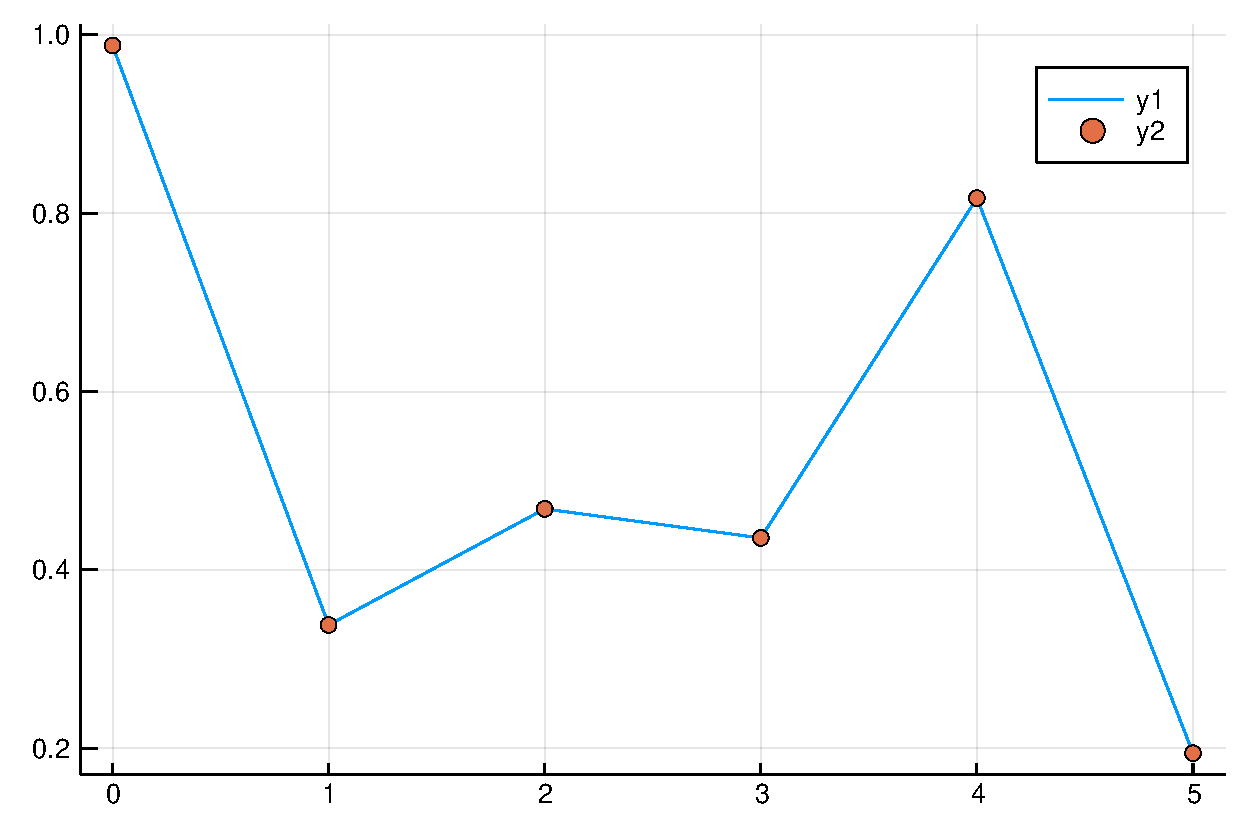
\includegraphics[height=0.66\textheight]{fig/plot2.pdf}
  \end{center}
\end{frame}


\begin{frame}[fragile]
  \frametitle{Overlaying plots, II}
  The \texttt{plot()} function creates a \emph{new} plot; \\
  the \texttt{plot!()} variant \emph{adds} to an existing one.

  \+
  You can also save a plot object to modify it later:
\begin{jl}
p = plot(xs, ys)
# ...
plot!(p, ...)
\end{jl}


  \+
  A number of functions are available to modify a plot's \textbf{attributes}:
  \texttt{title!}, \texttt{xlims!}, \texttt{xlabel!},
  \texttt{xticks!}, \texttt{ylims!}, \texttt{ylabel!}, etc.
\end{frame}


\begin{frame}[plain,fragile]
  \frametitle{Plotting functions, I}
\begin{semiverbatim}\small
\julia xs = -1:0.1:3; \lstinline|# from -1 to 3 in steps of 0.1|
\julia plot(xs, \HL{x->x^2})
\end{semiverbatim}
  \begin{center}
    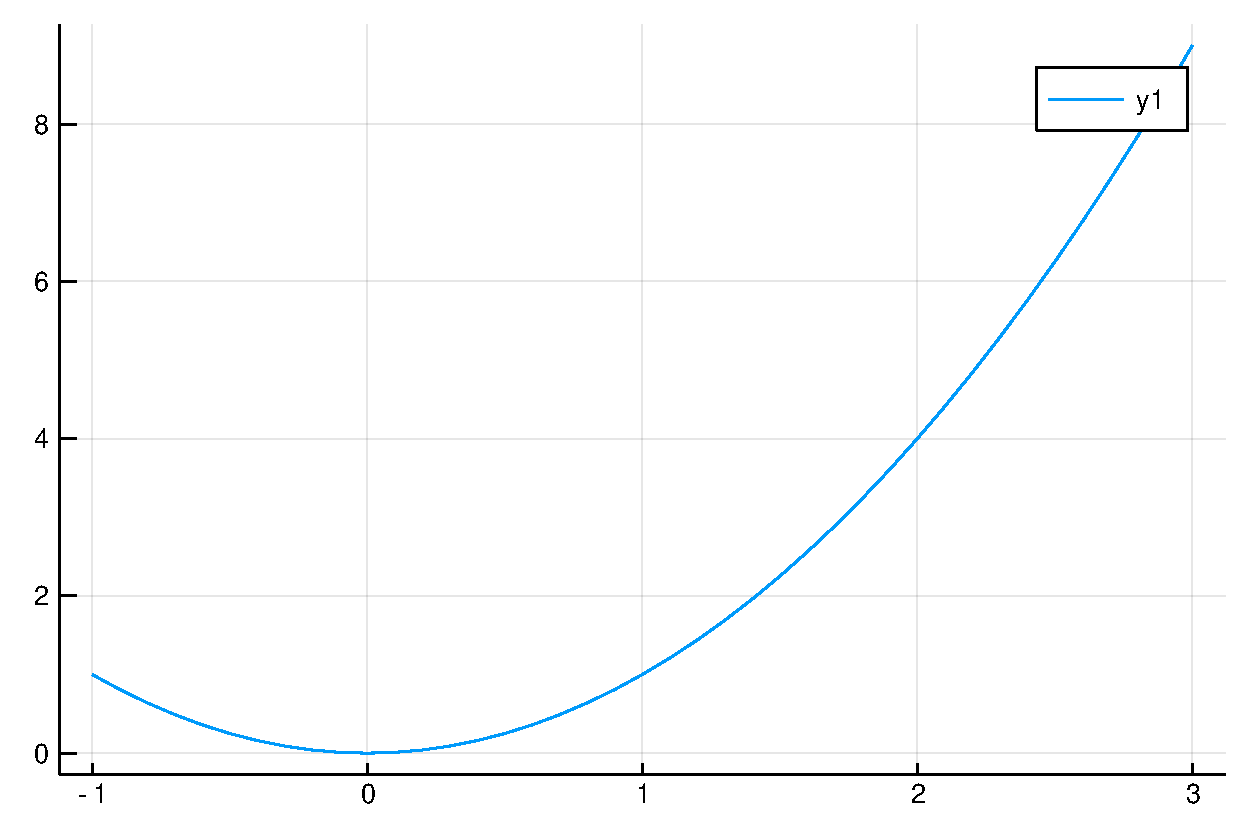
\includegraphics[height=0.60\textheight]{fig/plot3.pdf}
  \end{center}
  The $y$-axis coordinates can be a \emph{function} to compute the
  values from the $x$'s \ldots
\end{frame}


\begin{frame}[plain,fragile]
  \frametitle{Plotting functions, II}
\begin{semiverbatim}\small
\julia xs = -1:0.1:3;
\julia plot(xs, \HL{[x->x, x->x^2, x->cos(x)]})
\end{semiverbatim}
  \begin{center}
    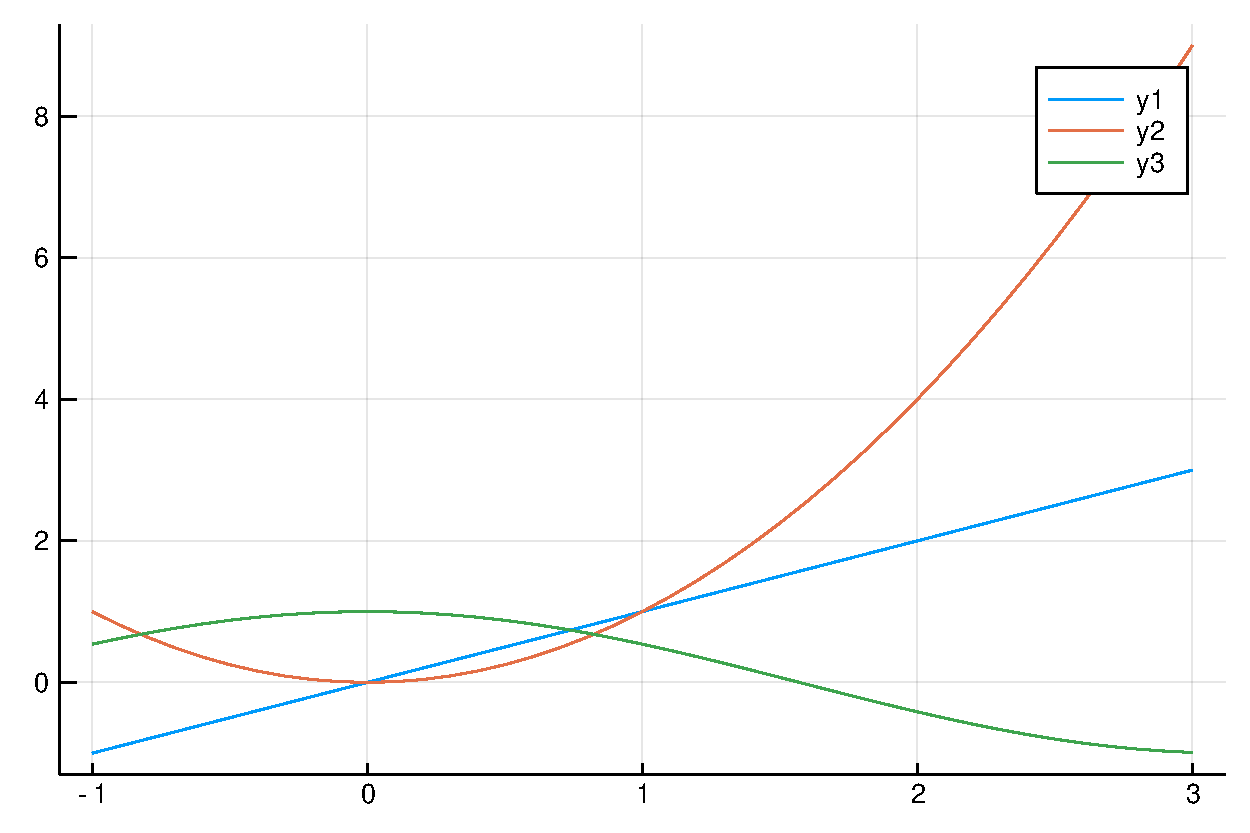
\includegraphics[height=0.60\textheight]{fig/plot4.pdf}
  \end{center}
  \ldots or a collection of functions!
\end{frame}


\begin{frame}
  \begin{exercise*}[4.A]
    Plot the graph of function $f(x) = 1/x$.

    Can you make the line 2 pixels thick?  Can you make the plot line
    red?
  \end{exercise*}

  \+
  \begin{exercise*}[4.B]
    Plot the functions $sin(x)$ and $2 \cdot cos(x) - 1$ on the
    interval $[-\pi, +\pi]$.

    How can you assign different attributes (e.g., line color) to the
    two lines?  For instance, color the $sin$ line red and the
    $cos$ line blue.
  \end{exercise*}

  \+
  \begin{exercise*}[4.C]
    Set \texttt{xs=-8:0.01:+8}; use \texttt{map} to collect the values
    of functions \texttt{sin(x)} and \texttt{cos(x)} into vectors
    \texttt{ys} and \texttt{zs}, respectively.

    Now evaluate \texttt{plot(xs, ys, zs)} --- what do you see?
    Does it work the same if you use the \texttt{sin} and \texttt{cos}
    functions instead of arrays \texttt{ys} and \texttt{zs}?
  \end{exercise*}
\end{frame}


\begin{frame}[fragile,fragile]
  \frametitle{Ranges, I}
  \small
  The notation $a:\delta:b$ denotes the collection of numbers $a$,
  $a+\delta$, $a+2\delta$, \ldots, $b$ (inclusive).

  \+
  When $\delta=1$, this can be abbreviated \texttt{$a$:$b$}.

  \+ Note that $b$ will be adjusted (towards 0) if $b-a$ is not an
  integral multiple of $\delta$:
\begin{semiverbatim}
\julia 0.5:0.25:2.3
0.5:0.25:2.25
\end{semiverbatim}

  \+
  The \texttt{collect()} function can be used to turn a range into a vector:
\begin{semiverbatim}
\julia collect(0.5:0.25:2.3)
8-element Array{Float64,1}:
 0.5
 0.75
 1.0
 \ldots
\end{semiverbatim}

\end{frame}


\begin{frame}[fragile]
  \frametitle{Ranges, II}
  The \texttt{range()} function allows a bit more flexibility:
\begin{lstlisting}
~\julia~ range(1, stop=5) # same as 1:5
1:5
~\julia~ range(1, stop=5, step=0.2) # same as 1:0.25:2.3
1.0:0.2:5.0
\end{lstlisting}

  \texttt{range()} allows specifying \texttt{stop=} and \texttt{step=}
  parameters in any order:
\begin{lstlisting}
~\julia~ range(0.5, step=0.25, stop=2.3)
0.5:0.25:2.25
\end{lstlisting}

  In addition, \texttt{range} allows automatically computing the step
  given a number of subdivisions:
\begin{lstlisting}
~\julia~ range(-1.0, stop=1.0, length=120)
-1.0:0.01680672268907563:1.0
\end{lstlisting}
\end{frame}


\part{Elementwise operations and Broadcasting}
\begin{frame}[fragile,fragile]
  \frametitle{Elementwise operations, I}
  For every binary operation like \texttt{*}, there is a corresponding ``dot''
  operation \texttt{.*} that is automatically defined to perform \texttt{*}
  element-by-element on arrays:
\begin{lstlisting}
~\julia~ v = [1,2,3];
~\julia~ v ~\HL{.*}~ v  # multiply elementwise
3-element Array{Int64,1}:
 1
 4
 9
\end{lstlisting}

  \+
  \begin{references}
    \url{https://docs.julialang.org/en/v1/manual/mathematical-operations/#man-dot-operators-1}
  \end{references}
\end{frame}

\begin{frame}[fragile]
  \frametitle{Elementwise operations, II}
  There is a corresponding ``dot'' notation for functions;
  note that the dot `\texttt{.}' goes \emph{after} the function name:
\begin{lstlisting}
~\julia~ xs = [0,1,2,3,5];
~\julia~ ys = ~\HL{cos.}~(xs)
5-element Array{Float64,1}:
  1.0
  0.5403023058681398
 -0.4161468365471424
 -0.9899924966004454
  0.28366218546322625
\end{lstlisting}
  There are no spaces between the function name (e.g.,~\texttt{cos})
  and the dot character.

  \+
  The dot notation can be applied to user-defined and built-in
  functions alike.

  \+
  \begin{references}
    \url{https://docs.julialang.org/en/v1/manual/mathematical-operations/#man-dot-operators-1}
  \end{references}
\end{frame}


\begin{frame}[fragile,fragile]
  \frametitle{Elementwise operations, III}
  A string of elementwise operations has a performance advantage: the
  Julia compiler can ``fuse'' multiple operations and make a
  single loop over the involved arrays, avoiding the creation
  of intermediate temporary storage places.

  \+
  An expression like:
\begin{lstlisting}
  ys = 2 ~\HL{.*}~ cos~\HL{.}~(xs) ~\HL{.-}~ 1
\end{lstlisting}
  is automatically unrolled into:
\begin{jl}
  temp = similar(xs)
  for i in 1:length(xs)
    temp[i] = 2*cos(xs[i]) - 1
  end
  ys = temp
\end{jl}

  \+
  \begin{references}
    \url{https://docs.julialang.org/en/v1/manual/functions/#man-vectorized-1}
  \end{references}
\end{frame}


\begin{frame}[fragile]
  \frametitle{Elementwise operations, IV}
  When combining multiple ``dot'' operations in a row, it is possible
  to use the \texttt{@.} macro to save typing and add readability.

  \+
  This expression:
\begin{lstlisting}
  ys = 2 ~\HL{.*}~ cos~\HL{.}~(xs) ~\HL{.-}~ 1
\end{lstlisting}
  can be rewritten as:
\begin{lstlisting}
  ys = ~\HL{@.}~ 2 * cos(xs) - 1
\end{lstlisting}

  \+
  \begin{references}
    \url{https://docs.julialang.org/en/v1/manual/mathematical-operations/#man-dot-operators-1}
  \end{references}
\end{frame}


\begin{frame}[fragile,fragile]
  \frametitle{Elementwise operations, V}
  \smaller
  The ``dotted assignment'' operator \texttt{.=} implements \textbf{in-place
    update} of an array: the array being assigned to is destructively
  replaced by values of the expression on the right-hand side.

  \+ For example, expression:
\begin{lstlisting}
  ys .= @. 2cos(xs)-1
\end{lstlisting}
  is internally rewritten as:
\begin{jl}
  for i in 1:length(xs)
    ys[i] = 2*cos(xs[i]) - 1
  end
\end{jl}

  \+ The macro \texttt{@allocated} allows checking how much memory is
  used for computing an expression:
\begin{lstlisting}
~\julia~ @allocated ys1 = @. 2cos(xs)-1
8000560
~\julia~ @allocated ys2 ~\HL{.=}~ @. 2cos(x)-1
480
\end{lstlisting}

  % \+
  % \begin{references}
  %   \url{https://docs.julialang.org/en/v1/manual/functions/#man-vectorized-1}
  % \end{references}
\end{frame}


\begin{frame}
  \smaller
  \begin{exercise*}[4.D*]
    Define three functions for computing the dot-product\footnote{In the
    linear algebraic sense.} of vectors:
  \begin{itemize}
  \item \texttt{dotprod1}: Use a \texttt{for}-loop and accumulate results;
  \item \texttt{dotprod2}: Use \texttt{.*} and the built-in function \texttt{sum()};
  \item \texttt{dotprod3}: Use function \texttt{dot} from the
    \texttt{LinearAlgebra} module.
  \end{itemize}

  \+
  Collect execution times (with the \texttt{@elapsed} macro) on a
  random vector of size $10^6$; how do they fare?

  \+
  Now collect allocation size (with the \texttt{@allocated} macro) on
  the same random vector; how does this compare to the running times?

  \+
  (To make things more interesting, you may want to collect times and
  allocation sizes on vectors of varying length and plot that data.)
  \end{exercise*}
\end{frame}


\begin{frame}[fragile]
  \frametitle{Broadcasting, I}
  ``Dotted'' operators allow mixing \\ scalars and arrays of different sizes:
\begin{lstlisting}
~\julia~ xs = 1:10;
~\julia~ ys = collect(1:10); # range->vector
~\julia~ plot(xs, [~\HL{ys .- 1}~, ys, ~\HL{ys .+ 1}~])
\end{lstlisting}
  \begin{center}
    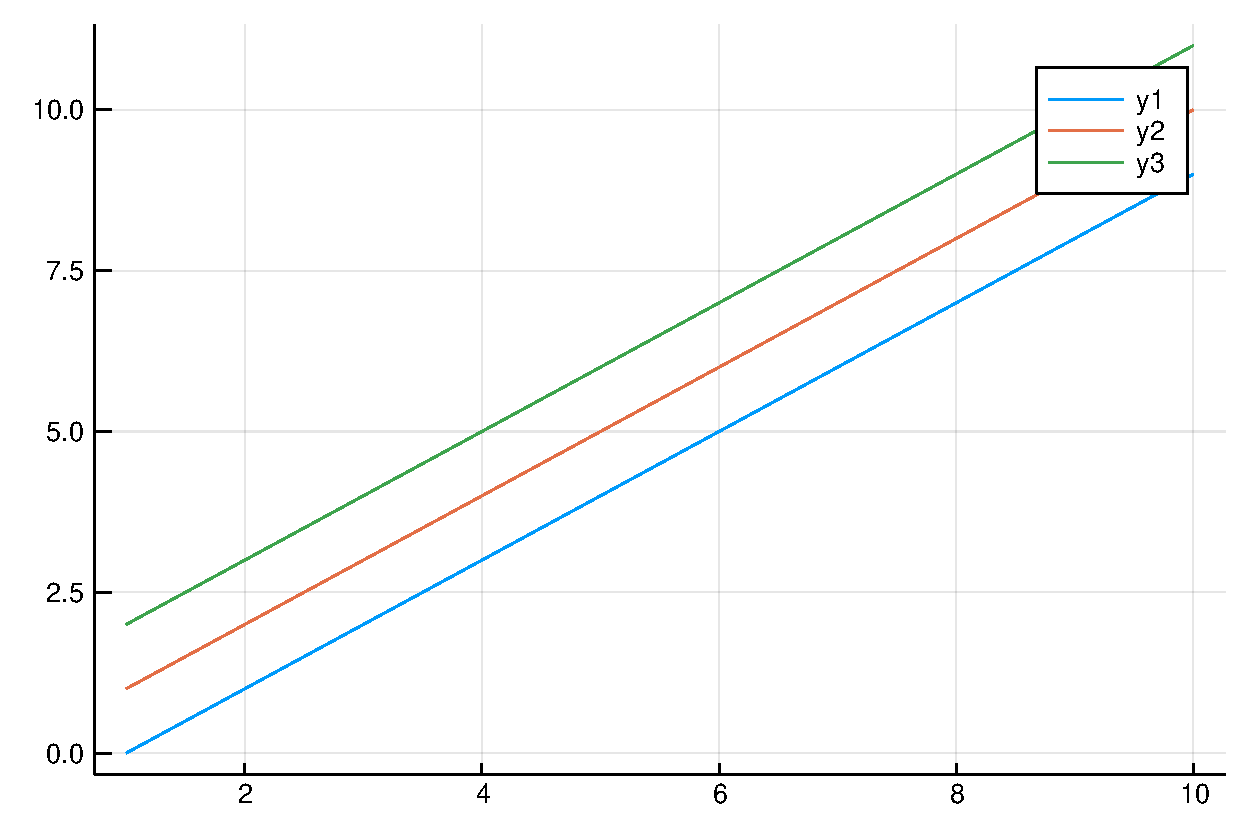
\includegraphics[height=0.50\textheight]{fig/plot5.pdf}
  \end{center}
\end{frame}


\begin{frame}[fragile]
  \frametitle{Broadcasting, II}
  \smaller
  When arrays of different sizes are mixed, Julia:
  \begin{itemize}
  \item \alert{replicates array values along missing axes,}
  \item expands singleton dimensions in array arguments
  \end{itemize}
  to match the other array:
\begin{semiverbatim}
\julia v = [1,2,3]  \lstinline|# column vector|
3-element Array\{Int64,1\}:
 1
 2
 3
\julia m = [1 2 3; 4 5 6; 7 8 9]
3×3 Array\{Int64,2\}:
 1  2  3
 4  5  6
 7  8  9
\julia m \HL{.+} v  \lstinline|# v[i] added to row i|
3×3 Array\{Int64,2\}:
  2   3   4
  6   7   8
 10  11  12
\end{semiverbatim}
\end{frame}


\begin{frame}[fragile]
  \frametitle{Broadcasting, III}
  \small
  When arrays of different sizes are mixed, Julia:
  \begin{itemize}
  \item replicates array values along missing axes,
  \item \alert{expands singleton dimensions in array arguments}
  \end{itemize}
  to match the other array:
\begin{semiverbatim}
\julia v'  \lstinline|# transpose -> row vector|
1×3 LinearAlgebra.Adjoint{Int64,Array{Int64,1}}:
 1  2  3
\julia m \HL{.*} v'  \lstinline|# v[i] muliplies column i|
3×3 Array{Int64,2}:
 1   4   9
 4  10  18
 7  16  27
\end{semiverbatim}
\end{frame}

% \begin{frame}[fragile,fragile]
%   \frametitle{Broadcasting, IV}
%   Broadcast also has a function form:
% \begin{semiverbatim}
% broadcast(f, a...)
% broadcast!(f, a...)
% \end{semiverbatim}
% \end{frame}

\begin{frame}
    \begin{exercise*}[4.E]
    Write a function \texttt{zscore(xs)} which, given a array
    \texttt{xs} of numbers, returns a similar array where every element
    has been normalized ($x \mapsto (x-\mu)/\sigma$) so that the
    result has mean 0 and std deviation 1.
  \end{exercise*}
\end{frame}


\part{Indexing}

\begin{frame}[fragile]
  \frametitle{Array indexing}

  When getting or setting array elements \texttt{m[i,~j,~k,~...]} each
  of the indices can be:
  \begin{itemize}
  \item a single scalar value --- selects only items whose corresponding
    coordinate is exactly that value;
  \item a range \texttt{$a$:$b$} --- selects items whose coordinate falls
    in the range;
  \item a strided range \texttt{$a$:$s$:$b$} --- selects items whose
    coordinate is one of $a$, $a+s$, \ldots, $b$;
  \item a boolean 1D array --- selects those items whose coordinate
    has the value \texttt{true} in the array.
  \end{itemize}
\end{frame}


\begin{frame}[fragile,fragile,fragile]
  \frametitle{Array indexing}
  \smaller
  Array slices can be used for getting or setting:
\begin{lstlisting}
~\julia~ using Statistics
~\julia~ v = randn(100);
~\julia~ q = quantile(v, 0.90);
~\julia~ i = (v .> q)  # need dotted comparison
100-element BitArray{1}:
 0
 0
 0
 1
~\ldots~
~\julia~ w = v[i]  # elements > q
10-element Array{Float64,1}:
 1.5486428522593445
 1.459431316814836
~\ldots~
\end{lstlisting}
  (This could be shortened as \texttt{w = v[v .> q]})
\end{frame}


\begin{frame}[fragile]
  \frametitle{Array indexing}
  Array slices can be used for getting or setting:
  \begin{columns}
    \begin{column}{0.6\textwidth}
\begin{lstlisting}
~\julia~ m = zeros(3, 3);
~\julia~ m[~\HL{:, 2}~] = ones(3);
~\julia~ m
3~$\times$~3 Array{Float64,2}:
 0.0  ~\HL{1.0}~  0.0
 0.0  ~\HL{1.0}~  0.0
 0.0  ~\HL{1.0}~  0.0
\end{lstlisting}
    \end{column}
    \begin{column}{0.6\textwidth}
\begin{lstlisting}
~\julia~ m = zeros(3, 3);
~\julia~ m[~\HL{1, :}~] = randn(3);
~\julia~ m
3~$\times$~3 Array{Float64,2}:
 ~\HL{0.5467  -0.0869  -1.2040}~
 0.0      0.0      0.0
 0.0      0.0      0.0
\end{lstlisting}
    \end{column}
  \end{columns}
\end{frame}


\begin{frame}[fragile]
  \frametitle{Array indexing}
  When assigning from a scalar value, or an array that does not match
  the shape of the one being assigned to, the dotted `\texttt{.=}'
  \emph{must} be used:
\begin{lstlisting}
~\julia~ checkers = [isodd(i+j)
                     for i in 1:3, j in 1:3];
~\julia~ m = zeros(Int, (3,3));
~\julia~ m[checkers] ~\HL{.=}~ 1;
~\julia~ m
3~$\times$~3 Array{Int64,2}:
 0  1  0
 1  0  1
 0  1  0
\end{lstlisting}
\end{frame}


\begin{frame}
  \begin{exercise*}[4.F]
    Write a function \texttt{cutoff!(a, q)} that given an array
    \texttt{a} and a percentage \texttt{q}, modifies \texttt{a} by
    setting all entries that are larger than the \texttt{q}-th
    percentile to exactly that value.  (You need to import package
    \texttt{Statistics} to access the \texttt{quantile()} function.)
  \end{exercise*}

  % \+
  % \begin{exercise*}[4.G*]
  %   Write a function \texttt{det(m)} which computes the determinant of
  %   (square) matrix \texttt{m}.
  % \end{exercise*}
\end{frame}


\part{Linear Algebra}
\begin{frame}
  \frametitle{Linear Algebra}
  The standard library \texttt{LinearAlgebra} provides:
  \begin{itemize}
  \item functions for calculations with vectors and matrices,
  \item matrix factorization (LU, DU, QR, etc.)
  \item specialized types for storing and computing with special matrices
  \end{itemize}

  \+
  \begin{references}
    \url{https://docs.julialang.org/en/v1/stdlib/LinearAlgebra/index.html}
  \end{references}
\end{frame}


\begin{frame}[fragile]
  \frametitle{Linear Algebra}
  Matrix-vector and matrix-matrix products are built-in the Julia core:
  \begin{columns}
    \begin{column}{0.5\textwidth}
\begin{lstlisting}
~\julia~ v = [1,2,3];
~\julia~ m
3~$\times$~3 Array{Int64,2}:
 0  1  0
 1  0  1
 0  1  0
~\julia~ m*v
3-element Array{Int64,1}:
 2
 4
 2
\end{lstlisting}
    \end{column}
    \begin{column}{0.5\textwidth}
\begin{lstlisting}
~\julia~ m*m
3~$\times$~3 Array{Int64,2}:
 1  0  1
 0  2  0
 1  0  1

~\julia~ m^2 + m
3~$\times$~3 Array{Int64,2}:
 1  1  1
 1  2  1
 1  1  1
\end{lstlisting}
    \end{column}
  \end{columns}
\end{frame}


\begin{frame}
  \frametitle{Linear Algebra}
  Other functions must be imported from \texttt{LinearAlgebra}:
  \smaller

  \+
  \begin{describe}{\texttt{dot(v,w)}, \texttt{cross(v,w)}}
      Dot- and cross-product of two vectors. \\
      (Also available in operator form \texttt{v$\cdot$ w} and \texttt{v
        $\times$ w}.)
  \end{describe}

  \+
  \begin{describe}{\texttt{tr(m)}, \texttt{det(m)}, \texttt{inv(m)}}
    Trace, determinant, and inverse of matrix \texttt{m}
  \end{describe}

  \+
  \begin{describe}{\texttt{eigvals(m)}, \texttt{eigvecs(m)}}
    Eigenvalues and Eigenvectors of matrix \texttt{m}
  \end{describe}

  \+
  \begin{describe}{\texttt{factorize(m)}, \texttt{lu(m)},
      \texttt{cholesky(m)}, etc.}
  Compute factorizations of matrix \texttt{m}.
  Function \texttt{factorize(m)} is the generic front-end that will
  compute a convenient factorization of \texttt{m}
  based on the actual ``shape''.
  \end{describe}
\end{frame}


\begin{frame}[fragile]
  \frametitle{Solving linear systems, I}
  The linear problem $Ax = b$ is solved by Julia's
  operator~`\texttt{\textbackslash}':
\begin{lstlisting}
~\julia~ a = randn((3,3));
~\julia~ v = [1,2,3];
~\julia~ x = a~\HL{\textbackslash}~v
3-element Array{Float64,1}:
  1.3909476657572728
 -3.398174579781128
  0.6163698662831701

~\julia~ a*x == v  # verify
true
\end{lstlisting}

 If matrix \texttt{a} is not square, Julia's `\texttt{a\textbackslash
   v}' returns the (minimum norm) least squares solution.
\end{frame}

\begin{frame}[fragile,fragile]
  \frametitle{Solving linear systems, II}
  Still, if a square matrix is not full-rank then an error is thrown:
\begin{lstlisting}
~\julia~ m = [0 1 0; 1 0 1; 0 1 0];
~\julia~ v = [1,2,3];
~\julia~ m\v
~\ERROR{SingularException(3)}~
\end{lstlisting}
\end{frame}


\part{Errors and exceptions}
\begin{frame}[fragile]
  \frametitle{Exceptions}

  ``Exceptions'' is the name given in to error conditions that cause a
  function to abort execution and signal the condition to the caller.

  \+
  If the caller cannot handle it, the exception is propagated up the
  call stack until a handler is found or the program exits.

  \+
  You can write code that intercepts some error conditions and
  reacts appropriately.

  \+
  \begin{seealso}
    \url{https://scls.gitbooks.io/ljthw/content/_chapters/11-ex8.html}
  \end{seealso}
\end{frame}


\begin{frame}[fragile]
  \frametitle{Handling exceptions}
\begin{lstlisting}
try
  # code that might raise an exception
catch err
  # handle some exception
finally
  # performed on exit in any case
end
\end{lstlisting}

  \+
  After a \texttt{catch} keyword, an optional name indicates a local
  variable that will hold the exception value --- code can inspect
  that to determine if and how to handle the exception.

  \+
  The optional \lstinline|finally| clause is executed on exit from the
  \lstinline|try| or \lstinline|catch| block in \emph{any} case.

  \begin{references}
    \smaller
    \url{https://docs.julialang.org/en/v1/base/base/#try}
\end{references}
\end{frame}


\begin{frame}[fragile]
  \frametitle{Handling exceptions, II}
  \small

  Julia's \texttt{try}/\texttt{catch} mechanism does not discriminate
  on the type of exception value thrown; it is completely up to the
  user to do that:
\begin{lstlisting}
try
  x = m\v;
catch err
  if isa(err, SingularException)
    @warn "Linear system is singular!"
    x = nothing;
  else
    # some other error happened, cannot handle
    rethrow() # propagate exception
  end
end
\end{lstlisting}

  The \texttt{rethrow} function, if called in a \texttt{catch} block,
  throws the current exception object, keeping the original throw location.
\end{frame}


\begin{frame}[fragile]
  \frametitle{Throwing exceptions}
  \smaller
  You can throw exceptions from your own code with these functions:

  \+
  \begin{describe}{\lstinline|error(msg)|}
    Raise an ErrorException with the given message.
  \end{describe}

  \+
  \begin{describe}{throw(err)}
    Throw a value as an exception.  Note that Julia does not enforce a
    specific type for exceptions --- any value will do!
  \end{describe}

  \+
  \begin{describe}{rethrow()}
    Throw an exception, without changing the backtrace (i.e., keeping
    the origin location intact).  If within a \texttt{catch} block,
    the exception value can be omitted and defaults to the exception
    being handled.
  \end{describe}

  \+
  \begin{references}
    \url{https://docs.julialang.org/en/v1/base/base/#Base.error}
  \end{references}
\end{frame}


\end{document}

%%% Local Variables:
%%% mode: latex
%%% TeX-master: t
%%% End:
